\chapter{Goals}

\section{Introduction}
Modern machine learning models based on deep neural networks are achieving remarkable performance on many fields, including medical image analysis. In comparison
with classic machine learning technologies like decision trees, it is much harder to explain how a neural network came to its conclusion, because it uses thousands to millions of training parameters.

In recent years, many methods for the interpretability of deep (convolutional) neural networks have been proposed, e.g. LIME\cite{ribeiro2016should}, RISE\cite{Petsiuk2018rise}, Grad-CAM\cite{selvaraju2017grad} or DeepLIFT \cite{shrikumar2017learning}.

\begin{figure}[h]
\centering
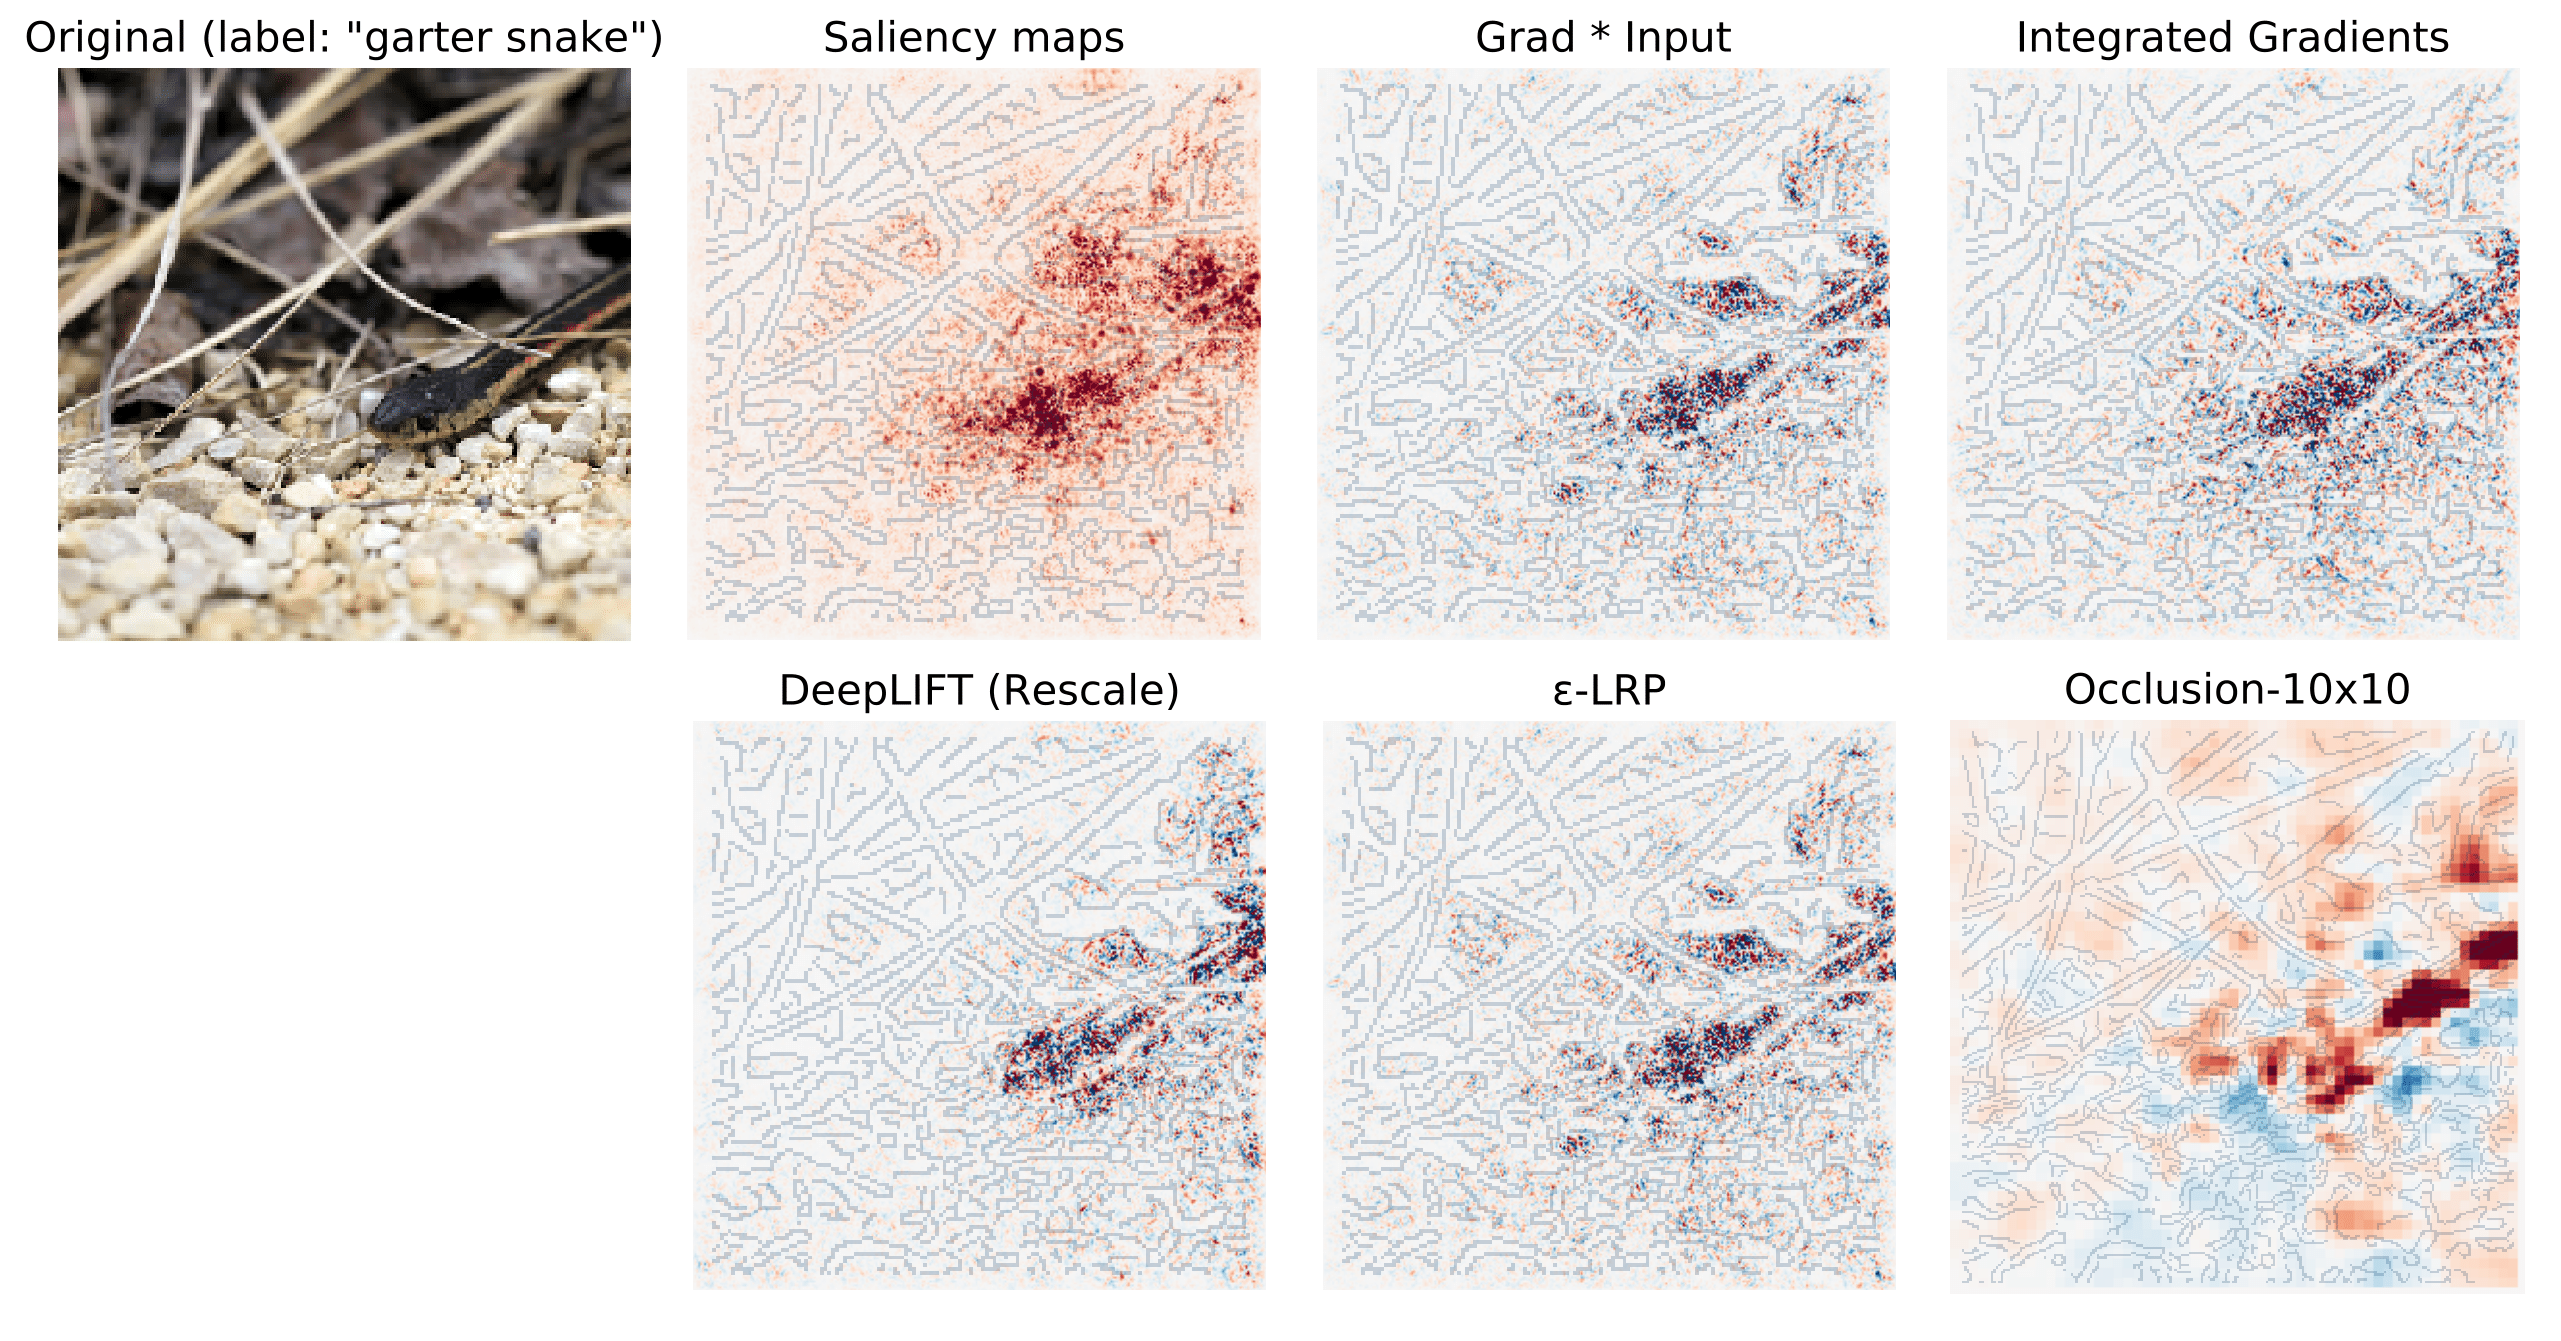
\includegraphics[width=14cm]{images/comparison.png}
\end{figure}

These methods focus on providing explanations and interpretability of classification problems for datasets like ImageNet or MNIST. What is missing is a method to interpret outputs of image segmentation problems.


\section{Infrastructure and technology}
This work will use the PyTorch\cite{paszke2017automatic} deep learning library. Most newer machine learning papers are written with PyTorch, because it is considered easier to learn and more powerful than Keras and PyTorch\cite{pytorchvstensorflow}.

Other machine learning libraries will be used on demand, for example:

\begin{tabular}{|p{3cm}|p{12.5cm}|}
    \hline
    \textbf{Library} & \textbf{Description} \\ \hline
    Scikit & Diverse kit of machine learning libraries \\ \hline
    Matplotlib & Library to generate graphs \\ \hline
    PIL/Pillow & Image manipulation library \\ \hline
    NumPy & Matrix manipulation library \\ \hline
    pandas & Dataframe library \\ \hline
    torchvision & PyTorch extension for computer vision problems. Contains models for common architectures and pretrained parameters for these networks. Also contains tools for data augmentation. \\ \hline
\end{tabular}

The development of the system will take place inside Jupyter notebooks. Jupyter notebooks allow a very fast test and development cycle. The notebook server will be running on a powerful desktop computer of the author which is exposed to the internet, so the computational power is always available independent of the work location.

In addition, the GPU servers from the Berner Fachhochschule (NVIDIA DGX-1, 4x Tesla V100) and from the Institute for Surgical Technology and Biomechanics of the Universität Bern (Unknown number and type of GPUs) are available. Because the setup cost to use these servers is quite high, the usage of these systems is optional and time will only be invested if the learning speedup is worth the additional setup time.

\section{Planning}
All steps described here are required to be completed if not marked otherwise. All steps build on the steps before it and cannot be skipped expect when explicitly mentioned.

\subsection{NIH Chest X-ray}
Purpose: Run some methods on a simpler dataset.
What is the dataset?
Used to figure out which methods work and can be used from PyTorch.
Use a basic image classificiation problem from the mediacal imaging field to evaluate methods.
\begin{itemize}
    \item Use the NIH chest x-ray dataset
    \item Learn a standard architecture for image classification on the model using PyTorch (e.g. Inception, ResNet)
    \item Apply methods on the output of the network
\end{itemize}


Goals
\begin{itemize}
    \item Determine which methods are directly usable with a PyTorch model or require low porting effort
    \item Determine which methods are independent of the used network architecture (methods that view the model as a black box)
    \item Find out how the output of the model looks like and (optionally) check with a medical professional which output they think would be most helpful
\end{itemize}


\subsection{Brain tumors}
The first thing we want to learn is the medical background of the thesis, answering the following questions:
\begin{itemize}
    \item What are brain tumors?
    \item What types of brain tumors exists?
    \item How do they look like on a scan? What scanner types exists (MRI/PET/CT)? Which one is used when?
    \item How does a scan look like? Colors? Layers? 2D/3D images?
    \item How does a doctor analyze such a scan?
\end{itemize}

\subsection{The BraTS dataset}
\begin{itemize}
    \item What scanner is used and what tumor types are detected?
    \item What data format is used to save the scans?
    \item In what format is the labeling saved?
    \item Build a loader for the dataset
    \item Display some scans
    \item Dataset: BraTS, extract 2D slices
    \item Do NOT use slice from same head in training \& validation set (they look nearly the same) 4 different labels, representing 4 different sizes of a tumor
    \item Merge innermost 2 layers into one
    \item an image has 4 black/white channels, use them as separate channels
\end{itemize}

\subsection{Model for the BraTS dataset}

\begin{itemize}
    \item Research current state of the art networks for image segmentation
    \item Investigate U-Net architectures
    \item Build and train network for the BraTS dataset in PyTorch based on an existing architecture
    \item Investigate and if necessary/helpful implement data augmentation for the dataset
\end{itemize}


\subsection{RISE}
Randomized Input Sampling for Explanations
Challenge: RISE works with classificatin, how can we remodel it to use segmentation output
Blackbox model
\begin{itemize}
    \item Investigate how RISE works
    \item Figure out how to use RISE in image segmentation tasks
    \item Implement RISE for the neural network implemented above
\end{itemize}

\subsection{Other blackbox model methods (Optional}
e.g. lime

\subsection{Grad-CAM Method}
Example for a whitebox model. Whitebox idea: dynamic unet can use standard model arch (e.g. resnet), so we can use these on half the network => does it make any sense?
Many implementations for PyTorch, an example for a whitebox model. If we get this to work, other methods should be possible too.

Do these methods work when we do not have a class? Only a specific activation?

Because this method is a whitebox model, it is independent of the implementation of the RISE model.


\subsection{Other whitebox model methods (Optional}

\subsubsection{iNNvestigate}
https://github.com/albermax/innvestigate

\begin{itemize}
    \item Figure out how to use iNNvestigate in image segmentation tasks
    \item Check if a port to 
\end{itemize}


\subsection{Library}
Build a library with a common interface for the implemented tools, so that all of them can be applied easily.
\begin{itemize}
    \item Write example programs for the library to use with PyTorch
    \item (Optional) Write example programs for the library to use with TensorFlow
    \item Write documentation how to use the library
    \item (Optional) Publish on conda
    \item (Optional) Publish on PyPI
    
\end{itemize}

\section{GANT Chart}
